\documentclass{article}
\title{Metodologia para escolha de um sensor de pasteurização}
\date{}

\usepackage[utf8]{inputenc}
\usepackage[portuguese]{babel}
\usepackage[margin=3.5cm]{geometry}
\usepackage{amsmath}
\usepackage{physics}
\usepackage{titlesec}
\usepackage{graphicx}
\usepackage{wrapfig}
\usepackage{caption}
\usepackage{subcaption}
\usepackage[parfill]{parskip}
\usepackage[nottoc]{tocbibind}
\usepackage[backend=biber]{biblatex}
\addbibresource{/home/luispengler/drive/LinuxFabrik/Research/read/bib.bib}
\usepackage{authblk}
\author[1]{Luís Spengler}
\affil[1]{Instituto Federal de Educação, Ciência e Tecnologia de Mato Grosso do Sul}

\begin{document}
\maketitle

\tableofcontents

\section{Introdução}
Pasteurização é um processo que consiste no aquecimento de um alimento a uma temperatura e depois o resfriamento da mesma, resultando em micro-organismos mortos. Industrias de diversos alimentos perecíveis poderiam se beneficiar de sistemas de automação da pasteurização.

\section{Problemática}
O problema aparece quando se faz o contrário: se encarrega de operadores humanos para controle da temperatura nas caldeiras, ocasionando em mão de obra mais cara e menor qualidade do processo. Com sistemas automatizados não haveria este risco, desde que estejamos utilizando um sensor com a exatidão que o processo requer.

\section{Objetivo Geral}
Determinar o sensor de temperatura infravermelho industrial mais adequado para a manutenção da temperatura constante a 100ºC e com menor variação possível.

\section{Metodologia}
No esquema abaixo, é representado o sistema de automação (sistema de controle de temperatura) a ser implementado na prática. Em temperaturas maiores que a expressão (100 + exatidão do sensor)ºC, o CLP manda um sinal para fechar a válvula (atuador) onde corre o GLP (gás liquefato de propano), em temperaturas menores que a expressão (100 - exatidão do sensor)ºC, o CLP manda um sinal para abrir a válvula (atuador) onde corre o GLP (gás liquefato de propano), fazendo com que a caldeira continue aquecendo e o processo repetido.
Procuramos então, um termômetro que atenda nossa especificação de boa exatidão, assim como repetibilidade e tempo de resposta adequados.

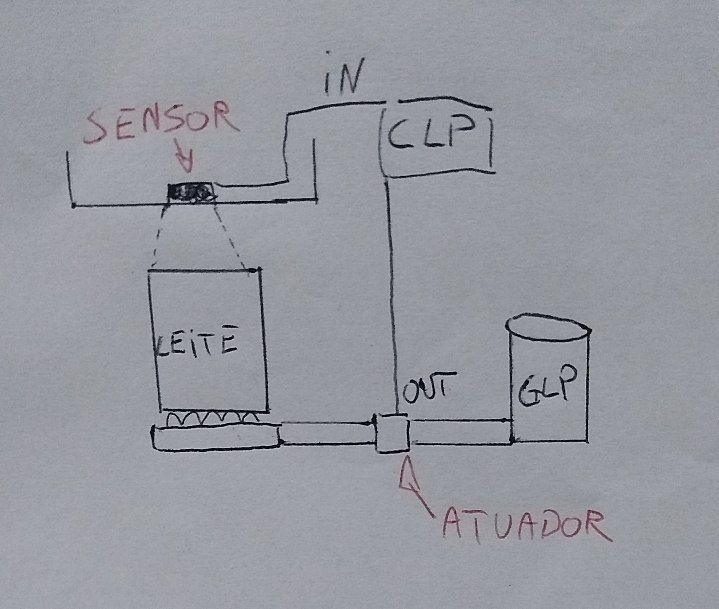
\includegraphics[scale=0.3]{esquema}


\section{Resultados}
No site Horiba.com é possível pesquisar termômetros industriais para diversas aplicações. Dentro os modelos comparados, o que mais atendia o requisitado, era o modelo IT-470F-H. Este possui uma precisão de 0,4ºC para mais e para menos e repetibilidade de 0,5ºC, ambos a temperatura de 100ºC. Seu tempo de resposta é adequado para a aplicação, ficando em torno de 1s em 95\% dos casos.

\section{Conclusão}
Pode-se concluir que o termômetro infravermelho industrial IT-470F-H se apresenta adequado para a implementação em um circuito de controle de temperatura para pasteurização a 100ºC.

\end{document}
